%%%%%%%%%%%%%%%%%%%%%%%%%%%%%%%%%%%%%%%%%%%%%%%%%%%%%%%%%%
%
% Doctoral Thesis Template @ The University of Manchester
% LaTeX Chapter Template
% Version 1 (23/07/2020)
% Joe Crone
%
% This template is based on:
% The University of Manchester, Presentation of Thesis Policy
% Research Office Graduate Education Team
% June 2017
% http://www.regulations.manchester.ac.uk/pgr-presentation-theses/
%
%%%%%%%%%%%%%%%%%%%%%%%%%%%%%%%%%%%%%%%%%%%%%%%%%%%%%%%%%%
\documentclass[../main.tex]{subfiles}
\begin{document}

% Title
%--------------------------------------------------------
\chapter{Introduction}
\label{Introduction} % to reference use \ref{ChapterTemplate}

Energy recovery Linacs (ERLs) are ideal drivers of inverse Compton scattering sources (ICS) due to the combination of linac quality beams and high repetition rate, allowing production of a tunable high-flux, narrowband scattered photon beam. The pioneering demonstration of multi-pass energy recovery in a superconducting RF (SRF) linac with FFAG return loop at the Cornell University Brookhaven National Laboratory Energy Recovery Linac Test Accelerator (CBETA) \cite{hoffstaetter2017cbeta} reveals a route to high energy electron beams for ERL driven ICS production of X-rays and $\gamma$-rays.

Due to a $E_{\gamma} \propto 4\gamma^{2}$ scattered photon energy $E_{\gamma}$ dependence, where $\gamma$ is the Lorentz factor, ICS is the prime candidate for production of high energy photons above photon energies available at conventional X-ray production facilities such as Free Electron Lasers (FEL)($E_{\gamma} <$~25~keV \cite{schneidmiller2011photon}) and the largest synchrotrons ($E_{\gamma} <$~500~keV) \textcolor{blue}{***Needs citation***}. Therefore, inverse Compton scattering sources are also the eminent method for high-flux production of $\gamma$-rays ($E_{\gamma} \sim$~1~MeV), which could support applications like nuclear resonance fluorescence (NRF) and nuclear photonics. ICS sources can be optimised to produce photons in smaller natural bandwidth than synchrotron radiation, alleviating the need for monochromators which inherently deplete the flux of the source. 

Experience gained this year from participating in CBETA commissioning and designing an X-ray ICS utilizing CBETA will ultimately motivate design choices and optimisations for an inverse Compton source operating on the posited Daresbury Industrial Accelerator for Nuclear Physics Applications (DIANA) ERL. The design values for the CBETA ICS are 4.64$\times 10^{8}$~ph/s in a 0.5\% bandwidth \textcolor{blue}{***Check flux figure hasn't changed***}up to a maximum photon energy of 401.4~keV. In comparison, the DIANA $\gamma$-ray source will be capable of producing $\sim 10^{11}$~ph/s in a 0.5\% bandwidth with scattered photon energies in the 1-20~MeV range, competitive with the flagship ELI-NP-GBS \cite{adriani2014technical} linac based inverse Compton scattering source. 

\section{The Cornell University -- Brookhaven National Laboratory Energy Recovery Linac Test Accelerator (CBETA)}

\begin{figure}[!htb]
\centering
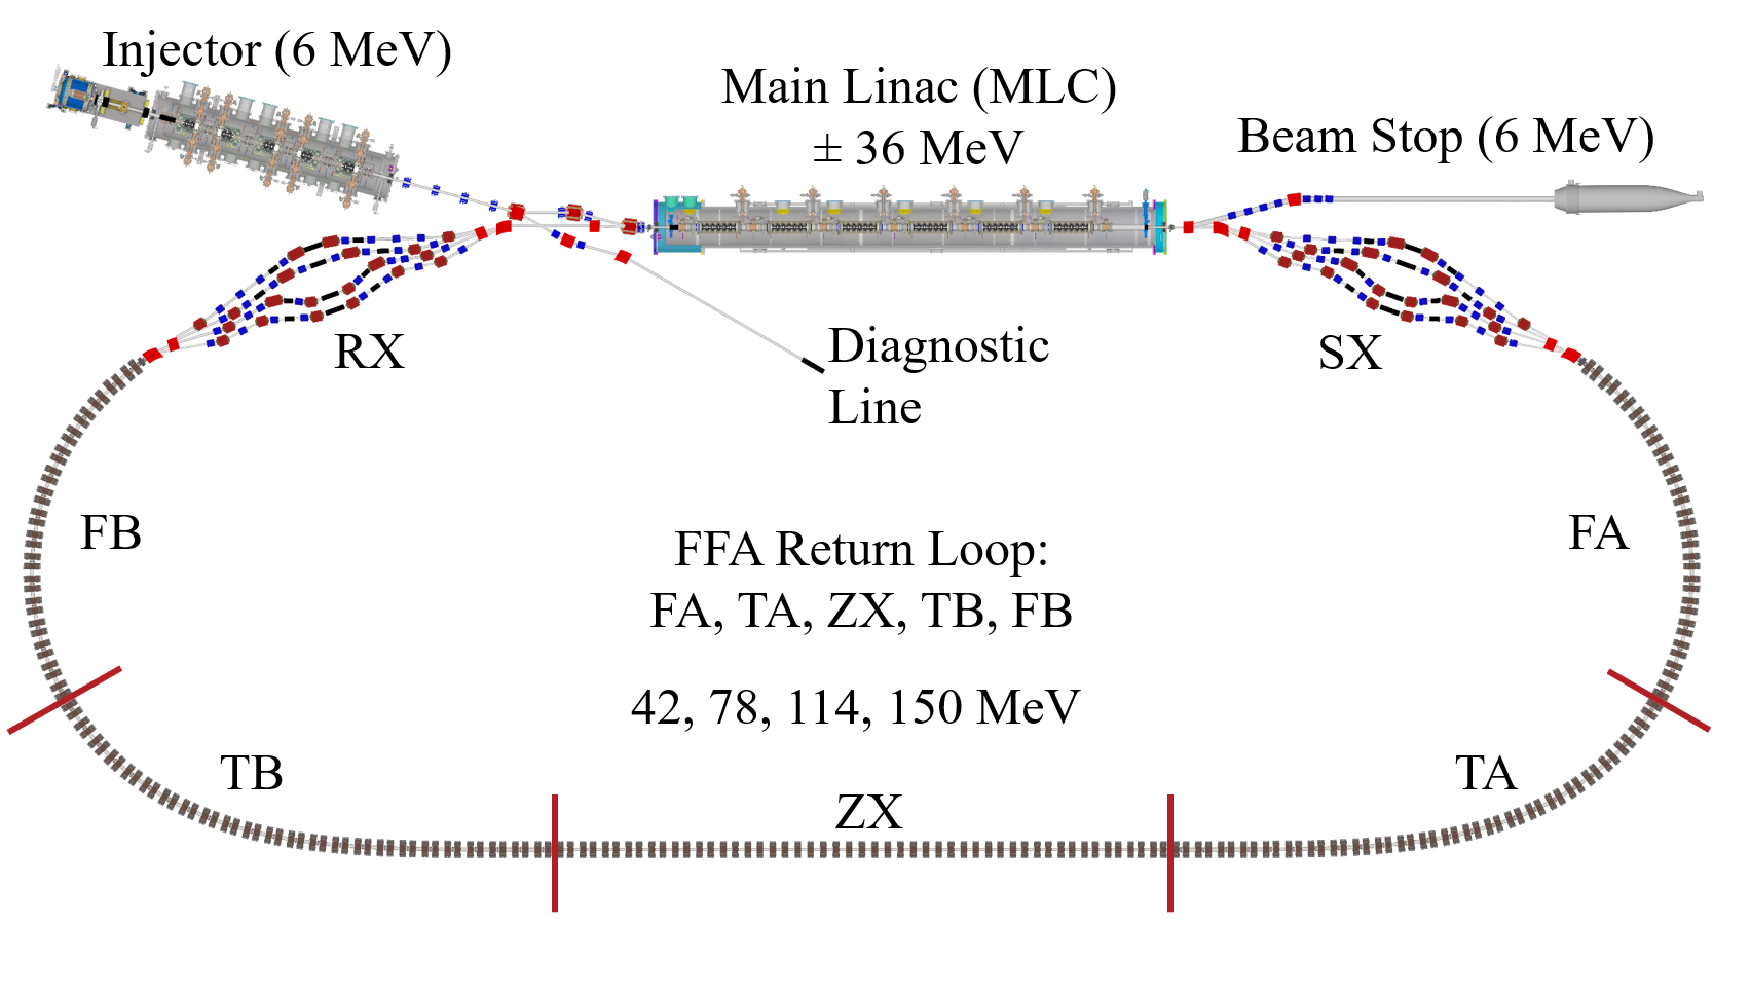
\includegraphics[width=\textwidth]{Figures/Introduction/CBETA_4pass_labels.pdf}
\caption{ Overview of the CBETA accelerator; a single FFA common transport arc (that includes the straight FFAsection ZX) carries all four beam energies (42, 78, 114, and 150 MeV) within a single beam pipe.  Matching of theentrance and exit beams at each energy is obtained through the SX and RX sections.}
\label{fig:CBETA_layout}
\end{figure}

\section{The Daresbury Industrial Accelerator for Nuclear Physics Applications (DIANA)}

\end{document}